\documentclass[12pt,letterpaper,english]{article}

\usepackage[margin=1.0in]{geometry}
\usepackage{helvetica}
\usepackage{graphicx}

\newcommand{\newpar}{\vspace{10mm}\noindent}

\title{An Analysis of Monsanto's Earning Announcement}
\author{Ian Clark}
\date{}

\begin{document}
\maketitle

\section{Results of the Earnings Report Upon the Market}
The market opened with news of Monsanto's Earnings Report readily available causing a rise--a $\Delta{P_{MON}} = 1.54 $--between the dates of 31 March 2015 closing and 01 April 2015 opening--01 April being the date where the earnings report was made available. There seemed to be a fair amount of inter day volatility within MON, as it reached a high of $117.13$ and a low of $113.62$. However, Monsanto ended the day trading near its high at $116.96$. As indicated by the chart below, we can see that Monsanto's stock price was much more volatile than in the nearly two weeks prior.

\newpar
\begin{center}
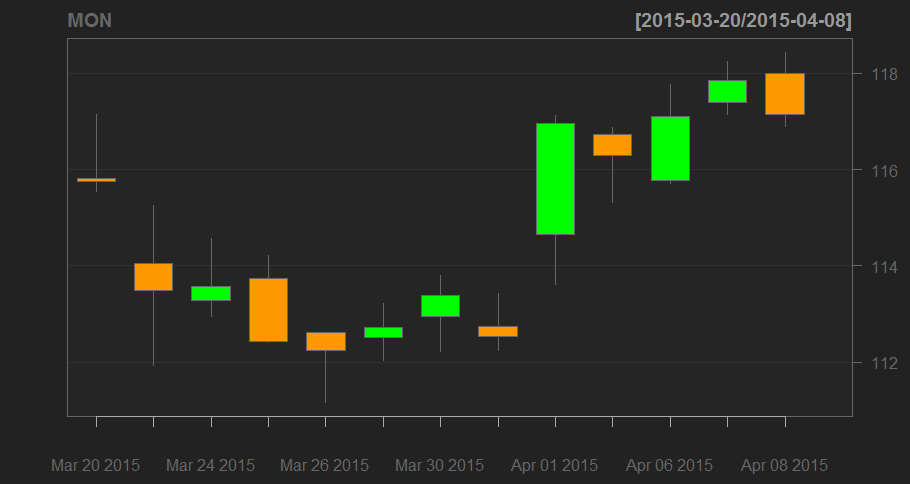
\includegraphics[scale=0.5]{Data/CandleChart.png}
\end{center}

\newpar
\subsection{Earnings per Share}
By Monsanto's estimates, their Earnings per Share ($2.92 \$ $) has remained within their estimates, but fallen over the course of the year toward the lower end of their acceptable range. A factor assumed to be heavily affecting both Monsanto and the US economy as a whole is the strengthening of the dollar in relations to other currencies--notably the Euro.

\newpar
In the second quarter of 2014, Monsanto reported an EPS of $3.15 \$ $. Therefore, Monsanto has realized a $\%\Delta{EPS} = -7$. Given that Monsanto still remains within their targeted range of EPS, this decrease, in and of itself, should not be too frightening for investors or potential investors. Although it may not be too frightening, the fact that the EPS has been decreasing for the previous two quarters indicates larger problems. As stated previously, the strengthening dollar has been causing ripples throughout the economy, Monsanto included.

\section{Growth}
While some of the more common metrics of growth may look less than promising, Monsanto has consistently been hitting milestones which will aide their future growth. In addition to this, one must consider general economic growth which has not looked too promising over the previous month. With a decreasing ISM and Monsanto announcing the missed acquisition of \textit{The Climate Corporation}, growth does look potentially hazardous in the near future; however, only time will truly tell how these two factors have been toward the future success and growth of Monsanto.

\subsection{Revenue Growth}
Monsanto announced net sales of nearly $5.2$ billion showing a decrease from net sales in the second quarter of 2014. While there may seem to be much negative news within this release, most of it appears to be noise given that both revenue growth and EPS are well within their previously established ranges. 

\subsection{Free Cash Flow}
As stated under the general growth section, Monsanto announced they missed the acquisition of \textit{The Climate Corporation}, thus leading them to have $986 \$$ million during their first two quarters of 2015 versus their $290 \$$ million during their first two quarters of 2014. While their Free Cash Flow is higher than both desired and expected, Monsanto seems earnest to ensure better future capital allocation. 

\section{Market Reactions}
As previously stated, the numbers as reported here have been within their estimated ranges and much of the variance between previous quarters has been explained by varying economic climates around the globe. As well, noise has been added due to the extraordinarily strong USD and ever weakening Euro.

\newpar
As for the validity of the market's reaction, everything seems reasonable: given their estimates have remained on course, their news was positive; therefore, the rising nature of the price was a reasonable market reaction. Moreover, the decreases within both the EPS and the net sales seem to be more noise-related than anything. However, there was a decent amount of variance in the inter day trading, as can be witnessed between the highs and lows of the stock's price. Much of this could be contributed by the realization of investors that while things are still looking decent, there may be issues with the economy as a whole.

\section{Personal Thoughts}
There have been ripples throughout the economy and stock markets due to various economic happenings, and as such, I feel most of the markets reactions to these stimuli have been reasonably received and neither overblown nor ignored. Ignoring the market, general economic conditions, and other various stimuli could produce many problems for the stock market either by overpricing stocks without considering the risk tied to a potential or even considerably looming recession. 

\newpar
While my view has been reasonably negative throughout this paper--reasonable in that I'm looking more toward general economic conditions than Monsanto--I feel that Monsanto has great opportunities for growth within their coming years, mostly due to the bolstered demand for Soy in the global and local (United States) markets. The only negative thing affecting my opinion of their future growth is them missing acquisitions--while not succeeding in all acquisitions is both expected and reasonable, I feel that their capital allocation is currently--not for the previous quarter--in-optimal.

\newpar
Going alongside my previous statement of in-optimality, Monsanto has postered themselves to, "focus on disciplined operational spend as a hedge to the current macro trends," which is very promising.
\newpage
\begin{thebibliography}{9}
\bibitem{Monsanto Earnings Presentation}
    Monsanto,
    \emph{$http://www.monsanto.com/investors/documents/2015/2015.04.01_mon_q2fy15_earnings.pdf$}.
\bibitem{Yahoo Finance Coverage of Report}
     Yahoo Finance,
     \emph{$http://finance.yahoo.com/news/monsanto-announces-second-quarter-financial-120000678.html$}
\end{thebibliography}

\end{document} 